\documentclass[usenames,dvipsnames]{beamer}
\usepackage{xcolor}
\usepackage{tikz}
\usepackage{listings}
\usepackage{algpseudocode}
\usefonttheme[onlymath]{serif}
\usepackage{amsmath}
\usetheme{Madrid}


\algnewcommand\algorithmicinput{\textbf{Input:}}
\algnewcommand\algorithmicoutput{\textbf{Output:}}
\algnewcommand\algorithmicinitialization{\textbf{Initialize:}}
\algnewcommand\Input{\item[\algorithmicinput]}%
\algnewcommand\Output{\item[\algorithmicoutput]}%
\algnewcommand\Initialize{\item[\algorithmicinitialization]}%


\logo{%
  \includegraphics[width=1cm,height=1.5cm,keepaspectratio]{Image/DUlogo}%
  \hspace{\dimexpr\paperwidth-2cm-5pt}%
  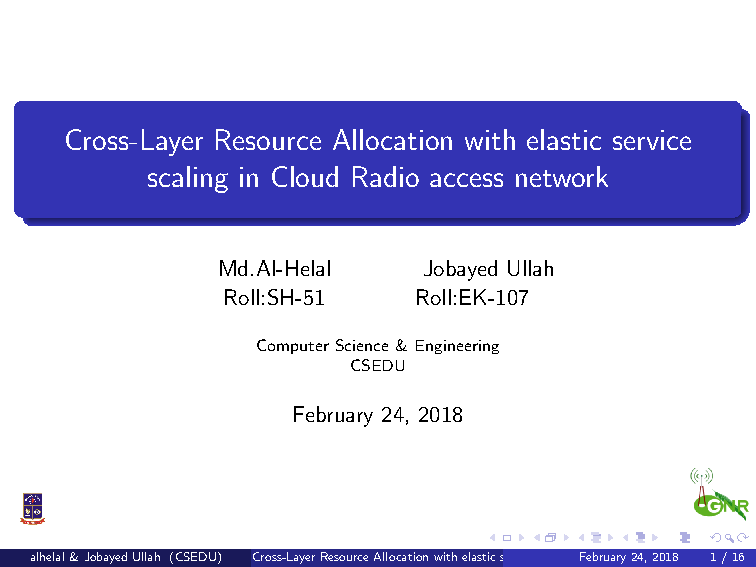
\includegraphics[width=1cm,height=1cm,keepaspectratio]{Image/GNR.png}%
}
\begin{document}
  \title{Cross-Layer  Resource  Allocation with  elastic service scaling in Cloud Radio access network}
  \author[alhelal \& Jobayed Ullah]{
  \parbox{2.5cm}{
\centering Md.Al-Helal\\Roll:SH-51}\hspace{1cm}
\parbox{2.5cm}{
{\centering Jobayed Ullah\\Roll:EK-107}}
}
\institute[CSEDU]{Computer Science \& Engineering\\CSEDU}
%\date{February 25, 2018}
\begin{frame}
  \maketitle
\end{frame}
  \title{Cross-Layer  Resource  Allocation with  elastic service scaling in Cloud Radio access network}
  \author{Jianhua Tang\\ Wee Pen Tay\\ Tony Q. S. Quek}
\institute{IEEE Transactions on Wireless Communications, vol 14, no. 9}
\date{September 2015}
\begin{frame}
  \maketitle
\end{frame}
  \author{alhelal \& Jobayed Ullah}
\institute{CSEDU}
\begin{frame}
  \frametitle{Assumption}
  \begin{exampleblock}{Assumption}
    \[
      \mu_{i},c_{i} > \lambda_{i}
    \]
    \[
      \varphi_{i}(\mu_{i})\geq 0, \forall \mu_{i}
    \]
    \[
      \varphi_{i}(\mu_{i}) \text{ is a convex and increasing function of } \mu_{i}
    \]
  \end{exampleblock}
  \begin{itemize}
    \item $\mu_{i}$\quad service rate
    \item $c_{i}$\quad transmission rate
    \item $\lambda_{i}$\quad arrival rate
    \item $\varphi_{i}{\mu_{i}} = k_{i}\mu_{i}^{a_{i}}$
    \item $k_{i} > 0$
    \item $a_{i} > 1$
  \end{itemize}
\end{frame}
\begin{frame}
  \frametitle{Aim}
  Minimizing system power consumtion in C-RAN, which consists of three components:
  \begin{itemize}
  \item Power consumption in BBU pool
  \item Power consumption in fibre links
  \item Power consumption in RRHs
  \end{itemize}
\end{frame}
\begin{frame}
  \frametitle{Delay equation}
  \begin{exampleblock}{Delay}
    \[
      d_{i} = \frac{1}{\mu_{i}- \lambda_{i}} + \frac{1}{c_{i} - \lambda_{i}}
  %    4545
    \]
  \end{exampleblock}
  \begin{itemize}
 % \centering
    \item  $d_{i}$\quad total delay
    \item $\mu_{i}$\quad service rate
    \item $\lambda_{i}$\quad arival rate
    \item $c_{i}$\quad transmission rate
  \end{itemize}
\end{frame}
\begin{frame}
  \frametitle{Equation}
  \begin{exampleblock}{Recieved signal at UE $i$}
    \[
      \hat{x_{i}} = \sum_{j\in{\mathcal{A}}}^{}h_{ij}^{H}w_{ij}x_{i} + \sum_{k\neq i}^{N}\sum_{j\in{A}}^{}h_{ij}^{H}w_{kj}x_{k} + \delta_{i}
    \]
  \end{exampleblock}
  \begin{itemize}
    \item $\mathcal{A}$\qquad set of active RRHs
    \item $x_{i}$\qquad data symbol for $i$th user
    \item $w_{ij}\in\mathbb{C}^{k}$\quad transmit beamformer for UE $i$ from RRH $j$
    \item $h_{ij}^{H}\in\mathbb{C}^{k}$\quad channel from RRH $j$ to UE $i$
    \item $\delta_{i}\sim\mathcal{C}\mathcal{N}(0,\sigma_{i})$\quad additive white Gaussian noise(AWGN) at UE $i$
    \item $i\in\mathcal{N}$
    \item $j\in\mathcal{A}$
  \end{itemize}
\end{frame}
\begin{frame}
  \frametitle{Equation}
  \begin{exampleblock}{Signal-to-Interference-plus-Noise-Ratio(SINR) at UE $i$}
    \[
%     \text{SINR}_{i}(A) = \frac{\lvert\sum_{j\in{A}}^{}h_{ij}^{H}w_{ij}\rvert^2}{\sigma_{i}^2 + \sum{k\neq i}^{N}
      \text{SINR}_{i}(\mathcal{A}) = \frac{\bigg\lvert\sum\limits_{j\in{\mathcal{A}}}^{}h_{ij}^{H}w_{ij}\bigg\rvert^2}{\sigma_{i}^2 + \sum\limits_{k\neq i}^{N}\bigg\lvert\sum\limits_{j\in{\mathcal{A}}}^{}h_{ij}^{H}w_{kj}\bigg\rvert}
    \]
  \end{exampleblock}
  \begin{itemize}
    \item $\sigma_{i}$
    \item $\mathcal{A}$\qquad set of active RRHs
    \item $w_{ij}\in\mathbb{C}^{k}$\quad transmit beamformer for UE $i$ from RRH $j$
    \item $h_{ij}^{H}\in\mathbb{C}^{k}$\quad channel from RRH $j$ to UE $i$
    \item $i\in\mathcal{N}$
    \item $j\in\mathcal{A}$
  \end{itemize}
\end{frame}
\begin{frame}
  \frametitle{Achieveable rate $c_{i}$}
  \begin{exampleblock}{The achieveable rate $c_{i}$ of UE $i$ should satisfy}
    \[
      c_{i} \leq B_{i}\log(1+\text{SINR}_{i}(\mathcal{A})) 
    \] 
  \end{exampleblock}
  \begin{itemize}
    \item $B_{i}$\qquad bandwidth for UE $i$\\
    \item SINR\quad Signal-to-Interference-plus-Noise-Ratio\\
    \item $\mathcal{A}$\qquad set of active RRHs
  \end{itemize}
\end{frame}
\begin{frame}
  \frametitle{Transmitting Power}
  \begin{exampleblock}{Each RRH $j$ has maximum transmitting power constraint}
    \[
      \sum_{i = 1}^{N}w_{ij}^{H}w_{ij}  = \sum_{i = 1}^{N} \lVert w_{ij}\rVert^2 \leq E_{j}
    \]
  \end{exampleblock}
  \begin{itemize}
    \item $w_{ij}\in\mathbb{C}^{k}$\quad transmit beamformer for UE $i$ from RRH $j$
    \item $i\in\mathcal{N}$
    \item $j\in\mathcal{L}$
  \end{itemize}
\end{frame}
\begin{frame}
  \frametitle{Optimization Problem}
  \vspace*{-2.5\baselineskip}
  \begin{columns}[t]
    \begin{column}{0.62\linewidth}
  \begin{exampleblock}{}
   \[
     \min_{\mu_{i},c_{i},w_{ij},\mathcal{A}}\sum_{i}^{N}\varphi_{i}(\mu_{i}) + \lvert\mathcal{A}\rvert P_{f} + \frac{1}{\eta}\sum_{i = 1}^{N}\sum_{j\in{A}}w_{ij}^{H}w_{ij}
   \]
  \end{exampleblock}
  subject to
  \begin{exampleblock}{}
    \[
      \frac{1}{\mu_{i}- \lambda_{i}} + \frac{1}{c_{i} - \lambda_{i}}\leq\tau_{i}
    \]
    \[
      \lambda_{i} < \mu_{i},\lambda_{i}<c_{i}
  %    4545
  \]
  \[
    c_i{i} \leq B_{i}\log(1+\text{SINR}_{i}(\mathcal{A}))
  \]
  \[
    \sum_{i=1}^{N}w_{ij}^{H}w_{ij}\leq E_{i},\quad \forall i\in \mathcal{N}, \quad \forall j\in \mathcal{L}
  \]
  \end{exampleblock}
\end{column}
\begin{column}{0.38\linewidth}
  \footnotesize\raggedright
  \begin{itemize}
    \item $\varphi_{i}(\mu_{i})$\quad VM $i$'s power consumption
    \item $\mu_{i}$\qquad VM $i$'s computation capacity/service rate/processing rate
    \item $P_{f}$\qquad power consumption active fibre links
    \item $\eta\in(0,1)$\quad ineffficiency coefficient amplifier in RRH
    \item $\mathcal{A}$\qquad set of active RRHs
    \item $w_{ij}\in\mathbb{C}^{k}$\quad transmit beamformer for UE $i$ from RRH $j$
    \item $i\in\mathcal{N}$
    \item $j\in\mathcal{A}$
  \end{itemize}
\end{column}
\end{columns}
\end{frame}
\begin{frame}
  \frametitle{QWSRM}
  \begin{exampleblock}{}
    \centering Quasi Weighted Sum-Rate Maximization Problem
  \end{exampleblock}
\end{frame}

\begin{frame}
  \frametitle{Quasi Weighted Sum-Rate Maximization Problem}
  \begin{exampleblock}{QWSRM}
    \[
      \min_{c_{i},w_{ij}} \sum_{i=1}^{N}-\varepsilon_{i}c_{i}
    \]
 % \end{exampleblock}
    subject to,
 % \begin{exampleblock}{}
    \[
      c_{i} \leq B_{i}\log(1+\text{SINR}_{i}(\mathcal{A})),\quad \forall i\in \mathcal{N}
    \]
    \[
      \sum_{i=1}^{N}w_{ij}^{H}w_{ij}\leq E_{i},\quad \forall j\in \mathcal{A}
    \]
  \end{exampleblock}
  \begin{itemize}
    \item $\varepsilon_{i}$\quad an arbitrary nonnegative weight
    \item $c_{i}$\quad transmission rate
    \item $B_{i}$\qquad bandwidth for UE $i$
    \item $\mathcal{A}$\qquad set of active RRHs
    \item $E_{j}$\quad maximum power on a link
    \item $w_{ij}\in\mathbb{C}^{k}$\quad transmit beamformer for UE $i$ from RRH $j$
    %\item SINR\qquad Signal-to-Interference-plus-Noise-Ratio
  \end{itemize}
\end{frame}

\begin{frame}
  \frametitle{Generalization of WSRM}
  \vspace*{-.5\baselineskip}
  \begin{exampleblock}{}
    \[
      \min_{c_{i},w_{ij}} f(\mathbf{c})
    \]
    subject to,
    \[
      \sum_{i=1}^{N}w_{ij}^{H}w_{ij}\leq E_{i},\quad \forall j\in \mathcal{A}
    \]
  \end{exampleblock}
  Where the objective function $f(\mathbf{c})$, for $0\leq\mathbf{c}\leq\bar{\mathbf{c}}$ has the following properties:
  \begin{itemize}
    \item $f(\mathbf{c})$ is a function only of $\mathbf{c}$, and
    \item $f(\mathbf{c})<\infty$ is continuously differentiable, and
    \item $f(\mathbf{c})$ is convex in the feasible region
    \item $\mathbf{c} = \begin{bmatrix}c_{1},\dots,c_{N}\end{bmatrix}^T$
    \item $w_{ij}\in\mathbb{C}^{k}$\quad transmit beamformer for UE $i$ from RRH $j$
    \item $c_{i}$\qquad transmission rate
    \item $E_{j}$\qquad maximum power on a link
    \item $\mathcal{A}$\qquad set of active RRHs
  \end{itemize}
\end{frame}
\begin{frame}[fragile]
  \footnotesize
    \begin{block}{BnB algorithm for QWSRM problem}
        \begin{algorithmic}

	  \Input $\mathcal{Q}_{\text{init}}, \mathcal{A}, \text{and} \mathcal{f} \text{(c)}.$
	  \Initialize Obtain $c_{i} \text{ by solving } \frac{\delta f(c)}{\delta c_{i}}=0, \text{ for } i\in\mathcal{N}.\text{ Set } k = 1, \mathcal{B} = \mathcal{Q}_{init},u_{1}=\gamma_{ub}(\mathcal{Q}_{init}) \text{ and } l_{1} = \gamma_{lb}(\mathcal{Q}_{init}).$\\
	  Check the feasibility of problem (17) with given
	  \If{feasible}
	  \State $c_{0} = \widetilde{c};$
	  \Else
	  \While{$u_{k} - l_{k} > \epsilon$}
	  \State Branching:
\State\quad\usebeamertemplate{itemize item} Set $\mathcal{Q}_{k} = \mathcal{Q}, \text{ where } \mathcal{Q} \text{ satisfies } \gamma_{lb}(\mathcal{Q}) = l_{k}.$
	  \State\quad\usebeamertemplate{itemize item} Split $\mathcal{Q} \text{ into } \mathcal{Q}_{\rm{I}} \text{ and } \mathcal{Q}_{\rm{II}}, \text{ along one of its longest edges.}$
	     \State\quad\usebeamertemplate{itemize item} Update $\mathcal{B}_{k+1} = (\mathcal{B}_{k}\setminus{\{\mathcal{Q}_{k}\}})\bigcup(\mathcal{Q}_{\rm{I}}, \mathcal{Q}_{\rm{II}}).$\\
	  \State Bounding:
	    \State\quad\usebeamertemplate{itemize item} Update $u_{k+1} = \min_{\mathcal{Q}\in\mathcal{B}_{k+1}}{\{\gamma_{ub}(\mathcal{Q})}\}$
\State\quad\usebeamertemplate{itemize item} Update $l_{k+1} = \min_{\mathcal{Q}\in\mathcal{B}_{k+1}}{\{\gamma_{lb}(\mathcal{Q})}\}$\\
	  \EndWhile\\
	  Set $c_{0} = c_{min};$
	  \EndIf
	  \Output $c_{0}.$
        \end{algorithmic}
    \end{block}
\end{frame}
\begin{frame}
 % \color{Brown}
  \color{Sepia}
  \centering \Huge\textbf{Thank You}
\end{frame}
\end{document}
